\documentclass{article}

\usepackage[left=2cm,right=2cm,top=2cm,bottom=2cm]{geometry} 

\usepackage[utf8]{inputenc}   % otra alternativa para los caracteres acentuados y la "ñ"
\usepackage[           spanish % para poder usar el español
                      ,es-tabla % para los captions de las tablas
                       ]{babel}   
\decimalpoint %para usar el punto decimal en vez de coma para los números con decimales

%\usepackage{beton}
%\usepackage[T1]{fontenc}

\usepackage{parskip}
\usepackage{xcolor}

\usepackage{caption}

\usepackage{fancyvrb}

\usepackage{enumerate} % paquete para poder personalizar fácilmente la apariencia de las listas enumerativas

\usepackage{graphicx} % figuras
\usepackage{subfigure} % subfiguras

\usepackage{amsfonts}
\usepackage{amsmath}

\usepackage[formats]{listings}
\lstdefineformat{R}{~=\( \sim \)}
\lstset{basicstyle=\ttfamily,format=R}

\definecolor{gris}{RGB}{220,220,220}
	
\usepackage{float} % para controlar la situación de los entornos flotantes

\restylefloat{figure}
\restylefloat{table} 
\setlength{\parindent}{0mm}


\usepackage[bookmarks=true,
            bookmarksnumbered=false, % true means bookmarks in 
                                     % left window are numbered
            bookmarksopen=false,     % true means only level 1
                                     % are displayed.
            colorlinks=true,
            allcolors=blue,
            urlcolor=blue]{hyperref}
\definecolor{webblue}{rgb}{0, 0, 0.5}  % less intense blue


\title{\Huge SWAP: Replicación de bases de datos MySQL\vspace{10mm}}

\author{\huge David Cabezas Berrido \vspace{10mm} \\ 
  \huge dxabezas@correo.ugr.es \vspace{10mm}}

\begin{document}
\maketitle
\tableofcontents
\newpage

\section{Preparativos}

Es importante desactivar el cortafuegos antes de hacer la configuración de maestro-esclavo. Como medida preventiva, desactivamos el 
cortafuegos en
todas las máquinas ejecutando el script \texttt{off.sh} de la práctica anterior (para \emph{iptables}) y también \verb|sudo ufw disable| (para UFW).

Como hicimos las reglas de \emph{iptables} permanentes, también ejecutamos (desde root)
\begin{Verbatim}
# iptables-save > /etc/iptables/rules.v4
\end{Verbatim}

\section{Base de datos MySQL}

Creamos la base de datos, la tabla e insertamos una tupla tal y como se describe en el guión.

Como opción avanzada, podemos exigir que algún campo no pueda ser nulo, por ejemplo el campo usuario. Esto se consigue
añadiendo \texttt{NOT NULL} detás del tipo del campo. Además, a la hora de insertar una tupla podemos omitir el nombre de los atributos si
 ponemos los valores en el mismo orden que aparecen en la descripción (el orden que usamos cuando creamos la tabla), aunque esto
 no es muy recomendable (si se modificase la tabla, habría que cambiar los scripts de inserción en caso de tenerlos).
 
\begin{figure}[H]
	\centering
	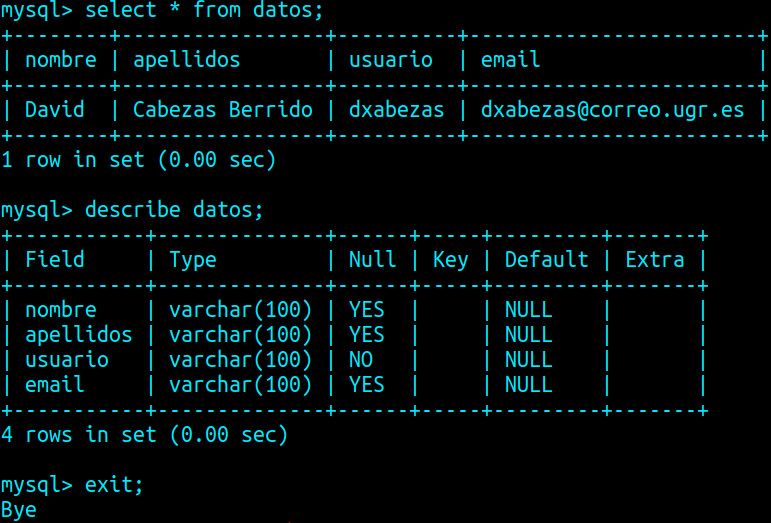
\includegraphics[width=120mm]{imgs/mydb}
	\caption{Tenemos una tupla en la tabla que hemos creado. En la descripción de la tabla podemos ver los distintos
	campos y el tipo de cada uno. Nos fijamos que el campo usuario no puede ser nulo (obtendremos un error si intentamos introducir
	una tupla con valor nulo para este atributo).}
	\label{fig:mydb}
\end{figure}

\subsection{Replicar la BD con mysqldump}

Antes de realizar la copia, debemos bloquear las tablas.

\begin{figure}[H]
	\centering
	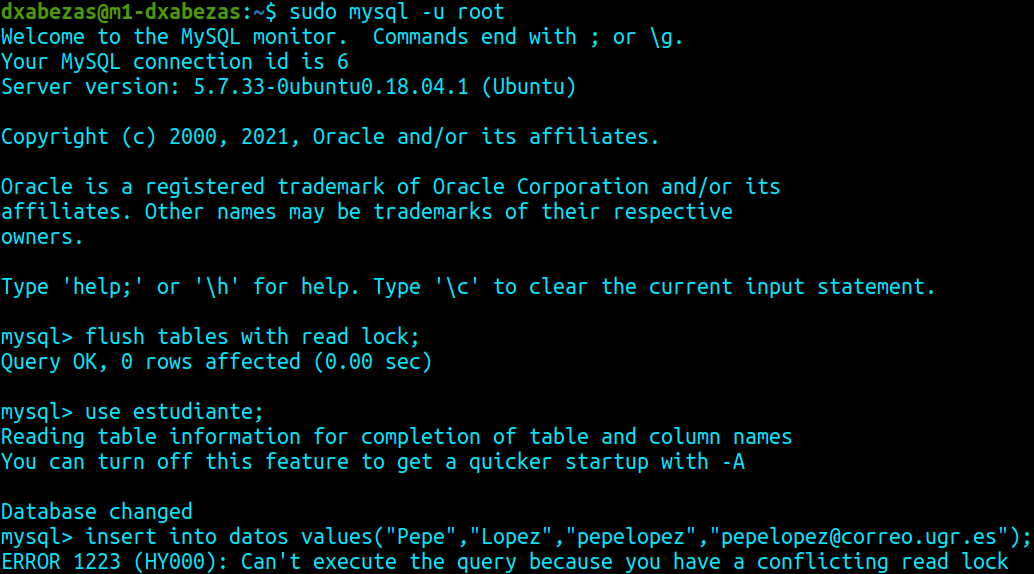
\includegraphics[width=150mm]{imgs/lock}
	\caption{Bloqueamos las tablas y comprobamos que no se puede modificar la base de datos.}
	\label{fig:lock}
\end{figure}

Ahora desde bash copiamos la base de datos a un archivo con
\begin{Verbatim}
sudo mysqldump estudiante -u root > /tmp/estudiante.sql
\end{Verbatim}
Después volvemos a entrar a MySQL y desbloqueamos las tablas con \verb|unlock tables;|. 

Copiamos el archivo a la máquina 2 (IP 192.168.56.101) con:
\begin{Verbatim}
sudo scp /tmp/estudiante.sql dxabezas@192.168.56.101:/tmp/estudiante.sql
\end{Verbatim}

A continuación, desde M2 creamos la base de datos al igual que hemos hecho en M1 (como se describe en el guión) y recuperamos
la copia con 
\begin{Verbatim}
sudo mysql -u root estudiante < /tmp/estudiante.sql
\end{Verbatim}
Si entramos a MySQL, podemos obtener el mismo resultado que en la Figura \ref{fig:mydb} (ahora en M2).

En el manual encontramos algunas opciones avanzadas que pueden ser útiles. Si tenemos varias bases de datos, podemos especificar
(tanto al copiar como restaurar)
las que queremos copiar con la opción \texttt{--databases <nombre-db1> <nombre-db2> \ldots} o usar \texttt{--all-databases} para
copiarlas todas. También podemos ahorrarnos tener que bloquear las tablas añadiendo la opción \texttt{--lock-all-tables} en el
\texttt{mysqldump} (para bloquear todas las tablas de todas las bases de datos) o simplemente \texttt{--lock-tables} para bloquear
sólo las tablas que copiamos. También podemos omitir las copias de algunas tablas con \texttt{--ignore-table=estudiante.datos} (en general, \texttt{<nombre db>.<nombre tabla>}) y omitir el contenido (las tuplas) de las tablas y copiar sólo la estructura con \texttt{--no-data}.

\section{Replicar la BD mediante configuración maestro-esclavo}

\subsubsection*{Configuración de MySQL del maestro (M1)}

Editamos como root el archivo \texttt{/etc/mysql/mysql.conf.d/mysqld.cnf} como se indica en el guión:
\begin{itemize}
	\item Comentamos \texttt{\#bind-address 127.0.0.1}.
	\item \texttt{log\_error = /var/log/mysql/error.log} (donde se almacena el log de errores).
	\item \texttt{server-id = 1}.
	\item \texttt{log\_bin = /var/log/mysql/bin.log} (donde se almacenan los binarios con la información).
\end{itemize}

Reiniciamos el servicio, todo parece estar correcto.
\begin{figure}[H]
	\centering
	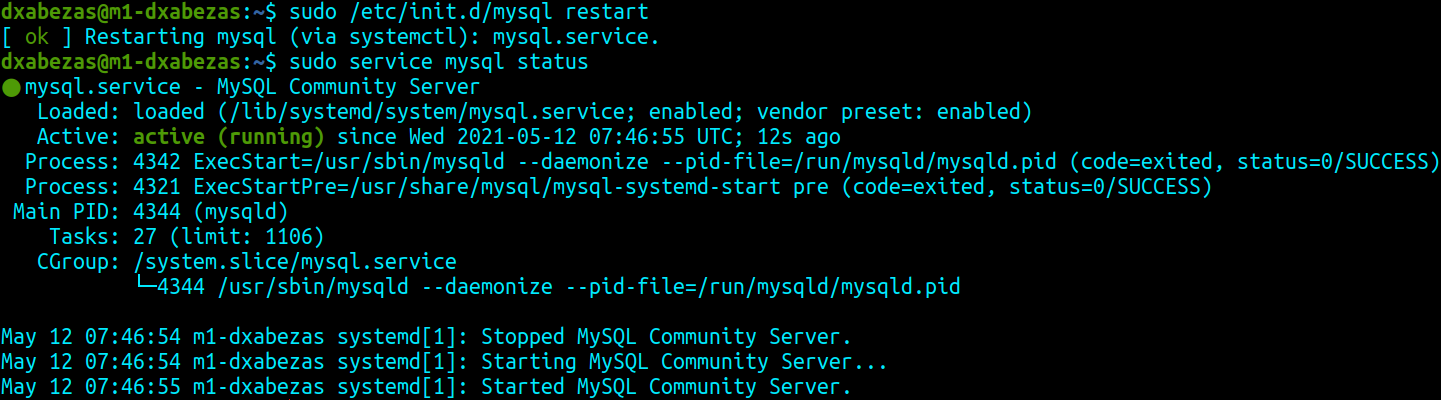
\includegraphics[width=170mm]{imgs/m1-mysql-restart}
\end{figure}

\subsubsection*{Configuración de MySQL del esclavo (M2)}
Hacemos las mismas configuraciones, pero con \texttt{server-id = 2}. Reiniciamos y comprobamos que también parece correcto.
\begin{figure}[H]
	\centering
	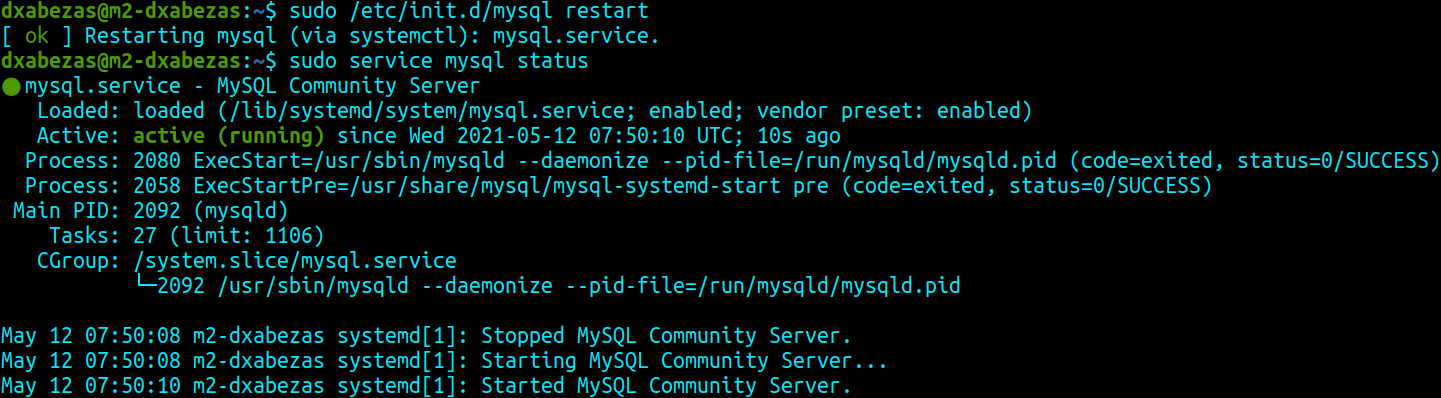
\includegraphics[width=170mm]{imgs/m2-mysql-restart}
\end{figure}

\subsubsection*{Configuración de MySQL del maestro (M1)}

Volvemos a M1, entramos a MySQL y creamos un usuario esclavo con los permisos necesarios para realizar la replicación y
bloqueamos las tablas.
\begin{Verbatim}
dxabezas@m1-dxabezas:~$ sudo mysql -u root

mysql> create user esclavo_dxabezas identified by 'esclavo_dxabezas';
mysql> grant replication slave on *.* to 'esclavo_dxabezas'@'%' identified by 'esclavo_dxabezas';
mysql> flush privileges;
mysql> flush tables;
mysql> flush tables with read lock;
\end{Verbatim}

A continuación, mostramos el estado del maestro.
\begin{figure}[H]
	\centering
	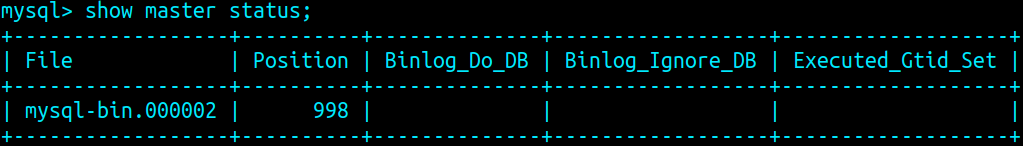
\includegraphics[width=150mm]{imgs/master-status}
\end{figure}
Estos datos son relativos a los ficheros de \texttt{log\_bin = /var/log/mysql/bin.log}, y cambian cuando
se realizan modificaciones. Por tanto, NO debemos tocar la base de datos hasta que no completemos la configuración.

\subsubsection*{Configuración de MySQL del esclavo (M2)}

Entramos a MySQL en M2, le damos los datos del maestro y arrancamos el esclavo.
\begin{Verbatim}[tabsize=7]
dxabezas@m2-dxabezas:~$ sudo mysql -u root

mysql> change master to master_host='192.168.56.102',
	master_user='esclavo_dxabezas', master_password='esclavo_dxabezas',
	master_log_file='mysql-bin.000002', master_log_pos=998, master_port=3306;
	
mysql> start slave;
\end{Verbatim}

\subsubsection*{Configuración de MySQL del maestro (M1)}
Volvemos una vez más a M1 para activar las tablas con
\begin{Verbatim}
dxabezas@m1-dxabezas:~$ sudo mysql -u root

mysql> unlock tables;
\end{Verbatim}

\subsubsection*{Configuración de MySQL del esclavo (M2)}
Comprobamos el estado del esclavo.
\begin{Verbatim}
dxabezas@m2-dxabezas:~$ sudo mysql -u root

mysql> show slave status\G;
\end{Verbatim}
Observamos que aparece \texttt{Seconds\_Behind\_Master: 0} y todos los marcadores de errores estan a 0 o son vacíos
(\texttt{Last\_SQL\_Error, Last\_IO\_Error, Last\_Error,\ldots}). Así que nos disponemos a probar la configuración introduciendo
nuevos datos en el maestro para ver si el esclavo los replica.

En M1, introducimos una nueva tupla.
\begin{Verbatim}
mysql> use estudiante;
mysql> insert into datos values("Pepe","Lopez","pepelopez","pepelopez@correo.ugr.es");
\end{Verbatim}
Y comprobamos que se ha añadido también en M2.
\begin{figure}[H]
	\centering
	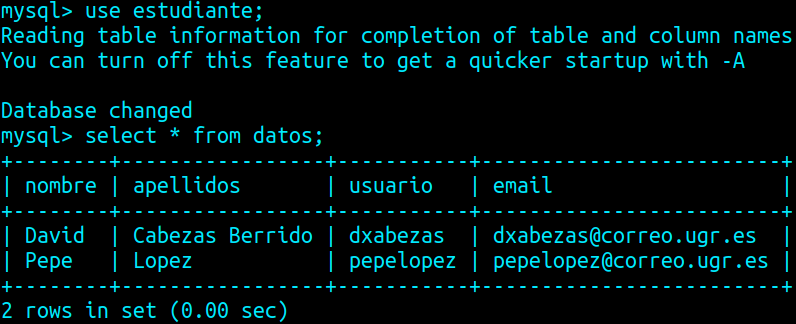
\includegraphics[width=140mm]{imgs/m2-master-slave}
	\caption{Base de datos de M2 tras añadir la tupla en M1.}
\end{figure}

Si nos fijamos, el estado del maestro ha cambiado.
\begin{figure}[H]
	\centering
	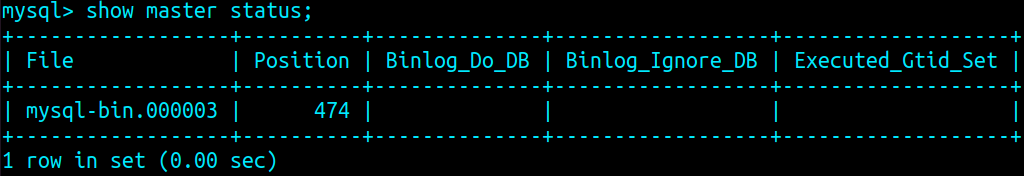
\includegraphics[width=150mm]{imgs/master-status2}
\end{figure}
Aunque los ficheros sean binarios, observamos secuencias relacionadas con las modificaciones que acabamos de hacer.
\begin{figure}[H]
	\centering
	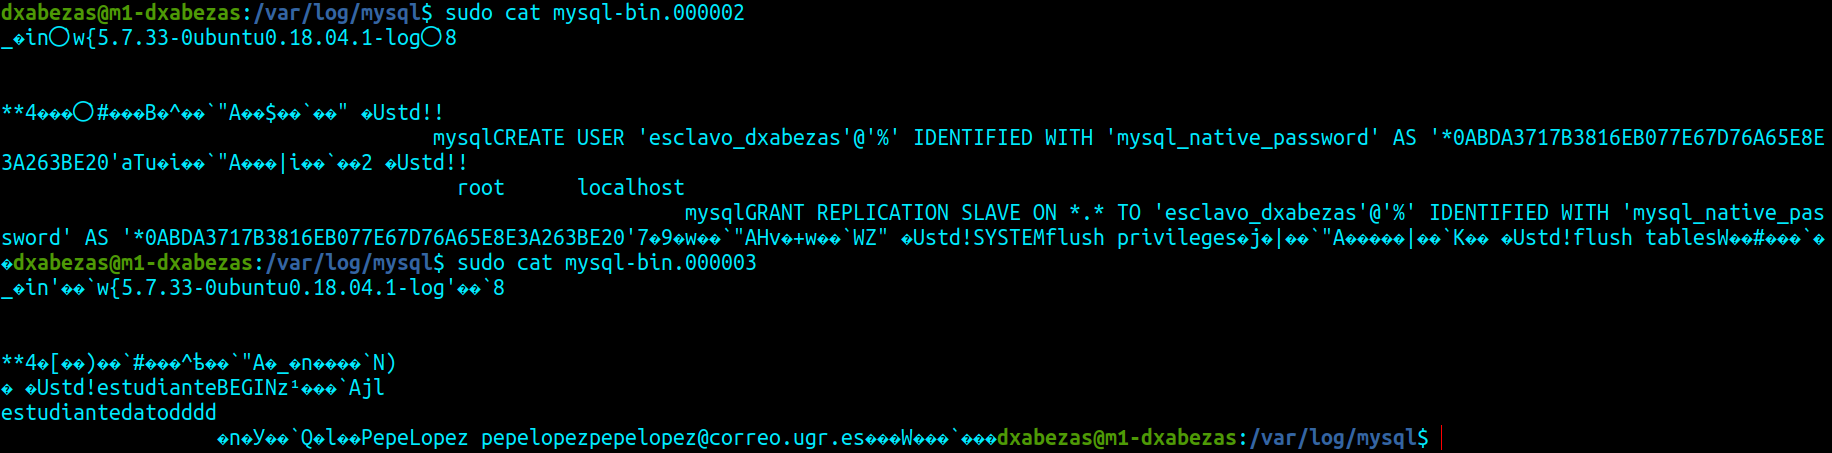
\includegraphics[width=170mm]{imgs/cat-bins}
\end{figure}

\section{Configurar \emph{iptables} para el puerto 3306}

TODO

\section{Replicar la BD mediante configuración maestro-maestro}

TODO

\end{document}
